\documentclass{article}

\title{Sistema de controle de mesa de som - Sistemas digitais e microcontrolados}
\date{}

\usepackage[utf8]{inputenc}
\usepackage[portuguese]{babel}
\usepackage[margin=2.5cm,headheight=0pt,headsep=0pt]{geometry}
\usepackage{amsmath}
\usepackage{physics}
\usepackage{xcolor}
\usepackage{titlesec}
\usepackage{graphicx}
\usepackage{wrapfig}
\usepackage{caption}
\usepackage{subcaption}
\usepackage{karnaugh-map}
\usepackage{setspace}
\usepackage[parfill]{parskip}
\usepackage[nottoc]{tocbibind}
\usepackage[backend=biber]{biblatex}
\addbibresource{/home/luispengler/drive/NextCloud/Research/read/bib.bib}
\usepackage{authblk}
\author[1]{Giovanna Bughi}
\author[2]{Gustavo Ratier Cardoso}
\author[3]{João Vitor Medeiros}
\author[4]{Luís Spengler}
\affil[1,2,3,4]{Instituto Federal de Educação, Ciência e Tecnologia de Mato Grosso do Sul}

\graphicspath{{./docs/}}

\renewcommand{\baselinestretch}{1.5}

\doublespacing

\usepackage{listings}
\lstset{%
  language = Octave,
  backgroundcolor=\color{white},
  basicstyle=\footnotesize\ttfamily,
  breakatwhitespace=false,
  breaklines=true,
  captionpos=b,
  commentstyle=\color{gray},
  deletekeywords={...},
  escapeinside={\%*}{*)},
  extendedchars=true,
  frame=single,
  keepspaces=true,
  keywordstyle=\color{orange},
  morekeywords={*,...},
  numbers=left,
  numbersep=5pt,
  numberstyle=\footnotesize\color{gray},
  rulecolor=\color{black},
  rulesepcolor=\color{blue},
  showspaces=false,
  showstringspaces=false,
  showtabs=false,
  stepnumber=2,
  stringstyle=\color{orange},
  tabsize=2,
  title=\lstname,
  emphstyle=\bfseries\color{blue}%  style for emph={}
}

%% language specific settings:
\lstdefinestyle{Arduino}{%
    language = Octave,
    keywords={void, int boolean},%                 define keywords
    morecomment=[l]{//},%             treat // as comments
    morecomment=[s]{/*}{*/},%         define /* ... */ comments
    emph={HIGH, OUTPUT, LOW}%        keywords to emphasize
}
\begin{document}

\begin{titlepage} % Suppresses displaying the page number on the title page and the subsequent page counts as page 1
	\newcommand{\HRule}{\rule{\linewidth}{0.5mm}} % Defines a new command for horizontal lines, change thickness here

	\center % Centre everything on the page

	%------------------------------------------------
	%	Headings
	%------------------------------------------------

	\textsc{\LARGE Instituto Federal de Educação, Ciência e Tecnologia de Mato Grosso do Sul}\\[1.5cm] % Main heading such as the name of your university/college

	\textsc{\Large Técnico em Eletrotécnica}\\[0.5cm] % Major heading such as course name

	\textsc{\large Disciplina de Sistemas Digitais e Microcontrolados}\\[0.5cm] % Minor heading such as course title

	%------------------------------------------------
	%	Title
	%------------------------------------------------

	\HRule\\[0.4cm]

	{\huge\bfseries ROTEIRO PARA ELABORAÇÃO DE PROJETO FINAL - Microcontrolador}\\[0.4cm] % Title of your document

	\HRule\\[1.5cm]

	%------------------------------------------------
	%	Author(s)
	%------------------------------------------------

	\vspace{30mm}
	\begin{minipage}{0.4\textwidth}
		\begin{flushleft}
			\large
			\textit{Autores}\\
			\textsc{Giovanna Bughi, Gustavo Ratier Cardoso, João Vitor Medeiros, Luís Spengler} % Your name
		\end{flushleft}
	\end{minipage}
	~
	
	% If you don't want a supervisor, uncomment the two lines below and comment the code above
	%{\large\textit{Author}}\\
	%John \textsc{Smith} % Your name

	%------------------------------------------------
	%	Date
	%------------------------------------------------

	\vfill\vfill\vfill\vfill\vfill\vfill\vfill % Position the date 3/4 down the remaining page
	
	{\large{Campo Grande, MS}\\
	\today} % Date, change the \today to a set date if you want to be precise

	%------------------------------------------------
	%	Logo
	%------------------------------------------------

	%\vfill\vfill
	%\includegraphics[width=0.2\textwidth]{placeholder.jpg}\\[1cm] % Include a department/university logo - this will require the graphicx package

	%----------------------------------------------------------------------------------------

	\vfill % Push the date up 1/4 of the remaining page

\end{titlepage}

\section{OBJETIVOS}
Desenvolvimento de Projetos Básicos Utilizando o Microcontrolador
\begin{itemize}
	\item[--] Projeto proposto: Controlador de Mesa de Som utilizando Microcontrolador
\end{itemize}
\section{Breve descrição do Projeto}
Para a mesa de som são conectados três microfones em uma única caixa de som amplificada, que são: ChP, ChD e ChC. A sigla “Ch” vem da palavra derivada do inglês, Channel (Canal), já as letras que à acompanham são do Presidente, Diretor e Coordenador, respectivamente. Foi identificado o nível de prioridade entre os microfones conforme sua transmissão e elaborado o circuito lógico combinacional que permitirá ligar os microfones segundo sua ordem de prioridade conforme a relação abaixo:

Prioridade 1: Presidente;

Prioridade 2: Diretor;

Prioridade 3: Coordenador.

Seu acionamento é simples, cada microfone é acionado pelo usuário através de um interruptor (liga-desliga) que nesse caso, serão também as entradas. Os microfones quando acionados comutam em sua saída 0 ou 1, informando ao circuito lógico que, por sua vez, aciona uma das saídas (SP, SD, SC) na caixa amplificada. Então, quando o Presidente ligar seu microfone, terá prioridade sobre os demais. Quando o Diretor ligar seu microfone, só terá prioridade sobre o Coordenador. E por fim, o Coordenador só falará quando os demais microfones não estiverem ligados.

\section{Foto e identificação do modelo do microcontrolador utilizado}
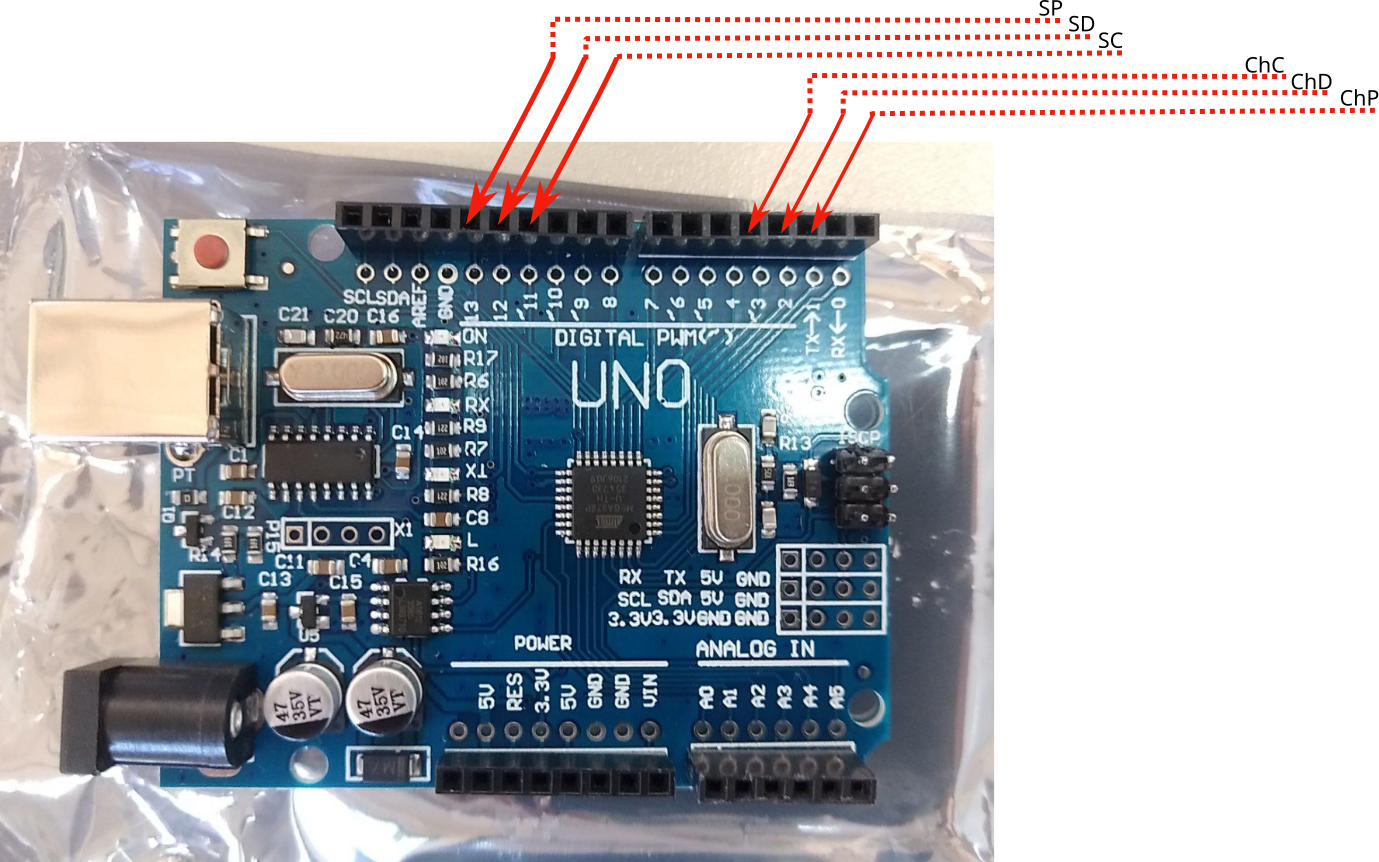
\includegraphics[width=\textwidth]{arduino}

\begin{itemize}
	\item MicroControlador: ATmega328
	\item Tensão de operação: 5V
	\item Tensão recomendada (entrada): 7-12V
	\item Limite da tensão de entrada: 6-20V
	\item Pinos digitais: 14 (seis pinos com saída PWM)
	\item Entrada analógica: 6 pinos
	\item Corrente contínua por pino de entrada e saída: 40 mA
	\item Corrente para o pino de 3.3 V: 50 mA
	\item Quantidade de memória FLASH: 32 KB (ATmega328) onde 0.5 KB usado para o bootloader
	\item Quantidade de memória SRAM: 2 KB (ATmega328)
	\item Quantidade de memória EEPROM: 1 KB (ATmega328)
	\item Velocidade de clock: 16 MHz
\end{itemize}

\section{Identificar e definir as  variáveis de entrada e saída}
Após a identificação do problema proposto, foram separadas e denominadas variáveis de entrada e saída que, serão utilizadas para a construção lógica e solução do problema. A entrada será referente ao canal de seus utilizadores, conforme sua prioridade; a letra S nas expressões lógicas é representada por saída e será utilizada para, denominar a saída do utilizador. A relação de entradas e saídas será:
\begin{itemize}
	\item Entradas – ChP, ChD e ChC;
	\item Saídas – SP, SD e SC.
\end{itemize}

\section{Definir os estados e condições das variáveis}
Nas entradas ChP, ChD e ChC terão nível lógico alto (1), somente quando os usuários tiverem seus microfones ligados; se todos tiverem seus microfones ligados: 
\begin{itemize}
\item ChP = 1, ChD = 1 e ChC = 1; 
\end{itemize}
em estado inicial todas as inicias serão iguais a zero (0), então: 
\begin{itemize}
	\item ChP = 0, ChD = 0, ChC = 0.
\end{itemize}
Conforme a conversa prossegue e os usuários ativam o microfone, são alteradas as variáveis de saída para estado lógico alto (1). A fim de determinar os estados de atuação em cada uma das entradas e saídas, preenchemos a tabela verdade de cada estado lógico, obedecendo a ordem de prioridade em cada falante de acordo com os valores da tabela abaixo:

\begin{displaymath}
\begin{array}{|c c c|c c c|}
INPUT & & & OUTPUT &\\
\hline
ChP & ChD & ChC & SP & SD & SC\\
\hline % Put a horizontal line between the table header and the rest.
0 & 0 & 0 & 0 & 0 & 0\\
0 & 0 & 1 & 0 & 0 & 1\\
0 & 1 & 0 & 0 & 1 & 0\\
0 & 1 & 1 & 0 & 1 & 0\\
1 & 0 & 0 & 1 & 0 & 0\\
1 & 0 & 1 & 1 & 0 & 0\\
1 & 1 & 0 & 1 & 0 & 0\\
1 & 1 & 1 & 1 & 0 & 0\\
\end{array}
\end{displaymath}

\section{Listar os comandos e instruções utilizados e sua sintaxe básica de operação}
Das linguagens que foram utilizadas para esse sistema, executarão a transmissão dos microfones conforme a prioridade estabelecida, demonstradas abaixo:

``define'' - É um componente do C++ que faz possível nomear um valor constante antes do programa ser compilado. Sintaxe:
\begin{lstlisting}[style=Arduino]
#define constantName value
\end{lstlisting}

``PinMode'' – É o modo em que as variáveis de entrada e saída serão identificadas pelo programa, quando ativado o sistema. Neste caso, o PinMode das entradas será configurado como “INPUT” (entrada) e configurado como “OUTPUT” (saída) para o PinMode das variáveis de saída. Sintaxe:
\begin{lstlisting}[style=Arduino]
pinMode(pin, mode);
\end{lstlisting}

``bool'' – Um ``bool'' só aceita um de dois valores, verdadeiro ou falso. (Cada variável ocupa um byte de memória). Sintaxe:
\begin{lstlisting}[style=Arduino]
bool var = val;
\end{lstlisting}

``DigitalRead'' – É o estado em que as variáveis, já definidas, serão identificadas em cada caso. Nas de entrada, o DigitalRead serve como alocação de memória para ser executado algum comando de acordo com a variável de saída; nas de saída, o DigitalRead irá comutar a saída desejada com o nível lógico programado (HIGH, se a saída é = 1 e LOW, se a saída é = 0). Sintaxe:
\begin{lstlisting}[style=Arduino]
digitalRead(pin)
\end{lstlisting}

``if'' – A função if (chamada de if statement) checa por uma condição e executa o código precedente ou conjunto deles se a condição é ‘verdadeira’. Sintaxe:
\begin{lstlisting}[style=arduino]
if (condition) {
  //code(s)
  } 
\end{lstlisting}

``DigitalWrite'' – Comuta valor HIGH ou LOW para a variável desejada. Sintaxe:
\begin{lstlisting}[style=arduino]
digitalWrite(pin, value)
\end{lstlisting}

\section{Firmware}
O código do arduino está abaixo
\begin{lstlisting}[style=Arduino]
#define SP 13
#define SD 12
#define SC 11
#define ChP 2
#define ChD 3
#define ChC 4

void setup() {
/* Saidas*/
  pinMode(SP, OUTPUT);
  pinMode(SD, OUTPUT);
  pinMode(SC, OUTPUT);
/* Entradas*/
  pinMode(ChP, INPUT);
  pinMode(ChD, INPUT);
  pinMode(ChC, INPUT);
}

void loop()
{
  bool Entp = digitalRead(ChP);
  bool Entd = digitalRead(ChD);
  bool Entc = digitalRead(ChC);
/* Se a chave do presidente estiver ligada...*/
  if (Entp)
  {
    digitalWrite(SP,HIGH); //Comutar a saida do presidente
    digitalWrite(SD,LOW);
    digitalWrite(SC,LOW);
  }
/* Se a chave do diretor estiver ligada
 *  e a chave do presidente estiver desligada...
 */
  if (Entd && !Entp)
  {
    digitalWrite(SP,LOW);
    digitalWrite(SD,HIGH); //Comutar a saida do diretor
    digitalWrite(SC,LOW);
  }
/* Se a chave do coordenador estiver ligada
 *  e a chave do diretor estiver desligada
 *  e a chave do presidente estiver desligada...
 */
  if (Entc && !Entd && !Entp)
  {
    digitalWrite(SP,LOW);
    digitalWrite(SD,LOW);
    digitalWrite(SC,HIGH); //Comutar a saida do coordenador
  }
/* Se o microfone de todos estiver desligado...*/
  if (!Entp && !Entd && !Entc)
  {
    digitalWrite(SP,LOW);
    digitalWrite(SD,LOW);
    digitalWrite(SC,LOW);
  }
}

\end{lstlisting}

\end{document}
